%%%%%%%%%%%%%%%%%%%%%%%%%%%%%%%%%%%%%%%%%
% University Assignment Title Page
% LaTeX Template
% Version 1.0 (27/12/12)
%
% This template has been downloaded from:
% http:\\www.LaTeXTemplates.com
%
% Original author:
% WikiBooks (http:\\en.wikibooks.org/wiki/LaTeX/Title_Creation)
%
% License:
% CC BY-NC-SA 3.0 (http:\\creativecommons.org/licenses/by-nc-sa/3.0/)
% %%%%%%%%%%%%%%%%%%%%%%%%%%%%%%%%%%%%%%%%
\documentclass[12pt]{article}
\usepackage{tabularx}
\usepackage[hidelinks]{hyperref}
\hypersetup{linktoc=all}

\usepackage{graphicx}
\graphicspath{{Resources/}}

\begin{document}
\sloppy

\begin{titlepage}

\newcommand{\HRule}{\rule{\linewidth}{0.5mm}} % Defines a new command for the
%horizontal lines, change thickness heReve

\center % Center everything on the page

%----------------------------------------------------------------------------------------
%	HEADING SECTIONS
%----------------------------------------------------------------------------------------

\textsc{\LARGE McMaster University}\\[1.5cm] % Name of your university/college
\textsc{\Large Software Project Management}\\[0.5cm] % Major heading such as course name
\textsc{\large SFWR ENG 3XA3}\\[0.5cm] % Minor heading such as course title

%----------------------------------------------------------------------------------------
%	TITLE SECTION
%----------------------------------------------------------------------------------------

\HRule \\[0.4cm]
{ \huge \bfseries Software Test Report}\\[0.4cm] % Title of your document
\HRule \\[1.5cm]

%----------------------------------------------------------------------------------------
%	AUTHOR SECTION
%----------------------------------------------------------------------------------------



% If you don't want a supervisor, uncomment the two lines below and remove the section above
\Large \emph{Authors:}\\
Mohammad \textsc{Naveed} \textbf{1332196} \\ % Your name
Josh \textsc{Voskamp} \textbf{1319352} \\
Stephan \textsc{Arulthasan} \textbf{1308004} \\[3cm]
%----------------------------------------------------------------------------------------
%	DATE SECTION
%----------------------------------------------------------------------------------------

{\large \today}\\[3cm] % Date, change the \today to a set date if you want to be precise

%----------------------------------------------------------------------------------------
%	LOGO SECTION
%----------------------------------------------------------------------------------------

%\includegraphics{Logo}\\[1cm] % Include a department/university logo - this will require the graphicx package

%----------------------------------------------------------------------------------------

\vfill % Fill the rest of the page with whitespace

\end{titlepage}

\newpage
\tableofcontents
\newpage
\listoftables
\addcontentsline{toc}{section}{List of Tables}
\newpage
\listoffigures
\addcontentsline{toc}{section}{List of Figures}
\newpage

\section*{Revision History}
\addcontentsline{toc}{section}{Revision History}
\begin{table}[!htbp]
	\centering
    \begin{tabular}{ | p{2cm} | l| l | l |p{3cm}|}
    \hline
    Revision Number & Revision Date & Description & Author \\ \hline
    0 & Nov 23 & Created Test Report & Josh Voskamp \\ \hline
	0 & Nov 23 & Intro, Scope, Methods & Stephan Arulthasan\\ \hline
    \end{tabular}
    \caption{Revision History}
\end{table}

\newpage

\section{Introduction}

\section{Testing Results}

\subsection{Test Case 1: Starting a new game}

\textbf{Initial State:} An existing game is running already. \\
\textbf{Input:} Escape Key\\
\textbf{Expected Output:} New game board initiated, with two random tiles with a value of 2 or 4 generated. \\
\textbf{Output:} New game board initiated, with two random tiles with a value of 2 or 4 generated \\
\textbf{Method of Testing:} Manual testing\\
\textbf{Pass/Fail:} Pass

\subsection{Test Case 2: Exiting a game}

\textbf{Initial State:} The game board is running already.\\
\textbf{Input:} User presses the red "X" that closes the window.\\
\textbf{Expected Output:} The window closes.\\
\textbf{Output:} The window closes. \\
\textbf{Method of Testing:} Manual testing\\
\textbf{Pass/Fail:} Pass

\subsection{Test Case 3: The user must be able to make moves}

\textbf{Initial State:} Game board is running with any set of tiles.\\
\textbf{Input:} User presses either of the 4 arrow keys.\\
\textbf{Expected Output:} The tiles move in the specified direction pressed by the user.\\
\textbf{Output:} The tiles move in the specified direction pressed by the user.
\textbf{Method of Testing:} Automated and Manual testing\\
\textbf{Pass/Fail:} Pass

\subsection{Test Case 4: The user must be able to win}

\textbf{Initial State:} The game board must be running with at least 2 1024 tiles beside
each other.\\
\textbf{Input:} The user presses one of the arrow keys that would join the two tiles together.\\
\textbf{Expected Output:} The two tiles join to create the 2048 tile and the game indicates the user has won. No more moves can be made.\\
\textbf{Output:} The two tiles join to create the 2048 tile and the game indicates the user has won. No more moves can be made.\\
\textbf{Method of Testing:} Automated and Manual testing\\
\textbf{Pass/Fail:} Pass

\subsection{Test Case 5: The user must be able to lose}

\textbf{Initial State:} The game board must be running in a state where the game board is full of tiles (16) with one more move available, which results in the next state having no more valid moves available, which means no two tiles that are the same are adjacent.\\
\textbf{Input:} User completes their only valid move\\
\textbf{Expected Output:} The game ends and displays "You Lose" message on screen.\\
\textbf{Output:} The game ends and displays "You Lose" message on screen.\\
\textbf{Method of Testing:} Automated and Manual testing\\
\textbf{Pass/Fail:} Pass

\subsection{Test Case 6: The user must not be able to move off the edge of the board}

\textbf{Initial State:} The game board must be running in a state where there is only one tile in the bottom left corner.\\
\textbf{Input:} User presses the left key.\\
\textbf{Expected Output:} Tile does not move off the left side of the board.\\
\textbf{Output:} Does not allow the tile to move left.\\
\textbf{Method of Testing:} Automated and Manual testing\\
\textbf{Pass/Fail:} Pass

\subsection{Test Case 7: Testing against Existing Implementation.}
\textbf{Initial State:} Original implementation and new implementation, with idential tile locations\\
\textbf{Input:} User performs the same action on both implementations\\
\textbf{Expected Output:} Both implementations result in the same board except for the new randomly generated tile\\
\textbf{Output:} Both implementations result in the same board except for the new randomly generated tile\\
\textbf{Method of Testing:} Manual testing, compare the resulting board from each implementation of the game\\
\textbf{Pass/Fail:} Pass

\begin{figure}[!htbp]
	\centering
	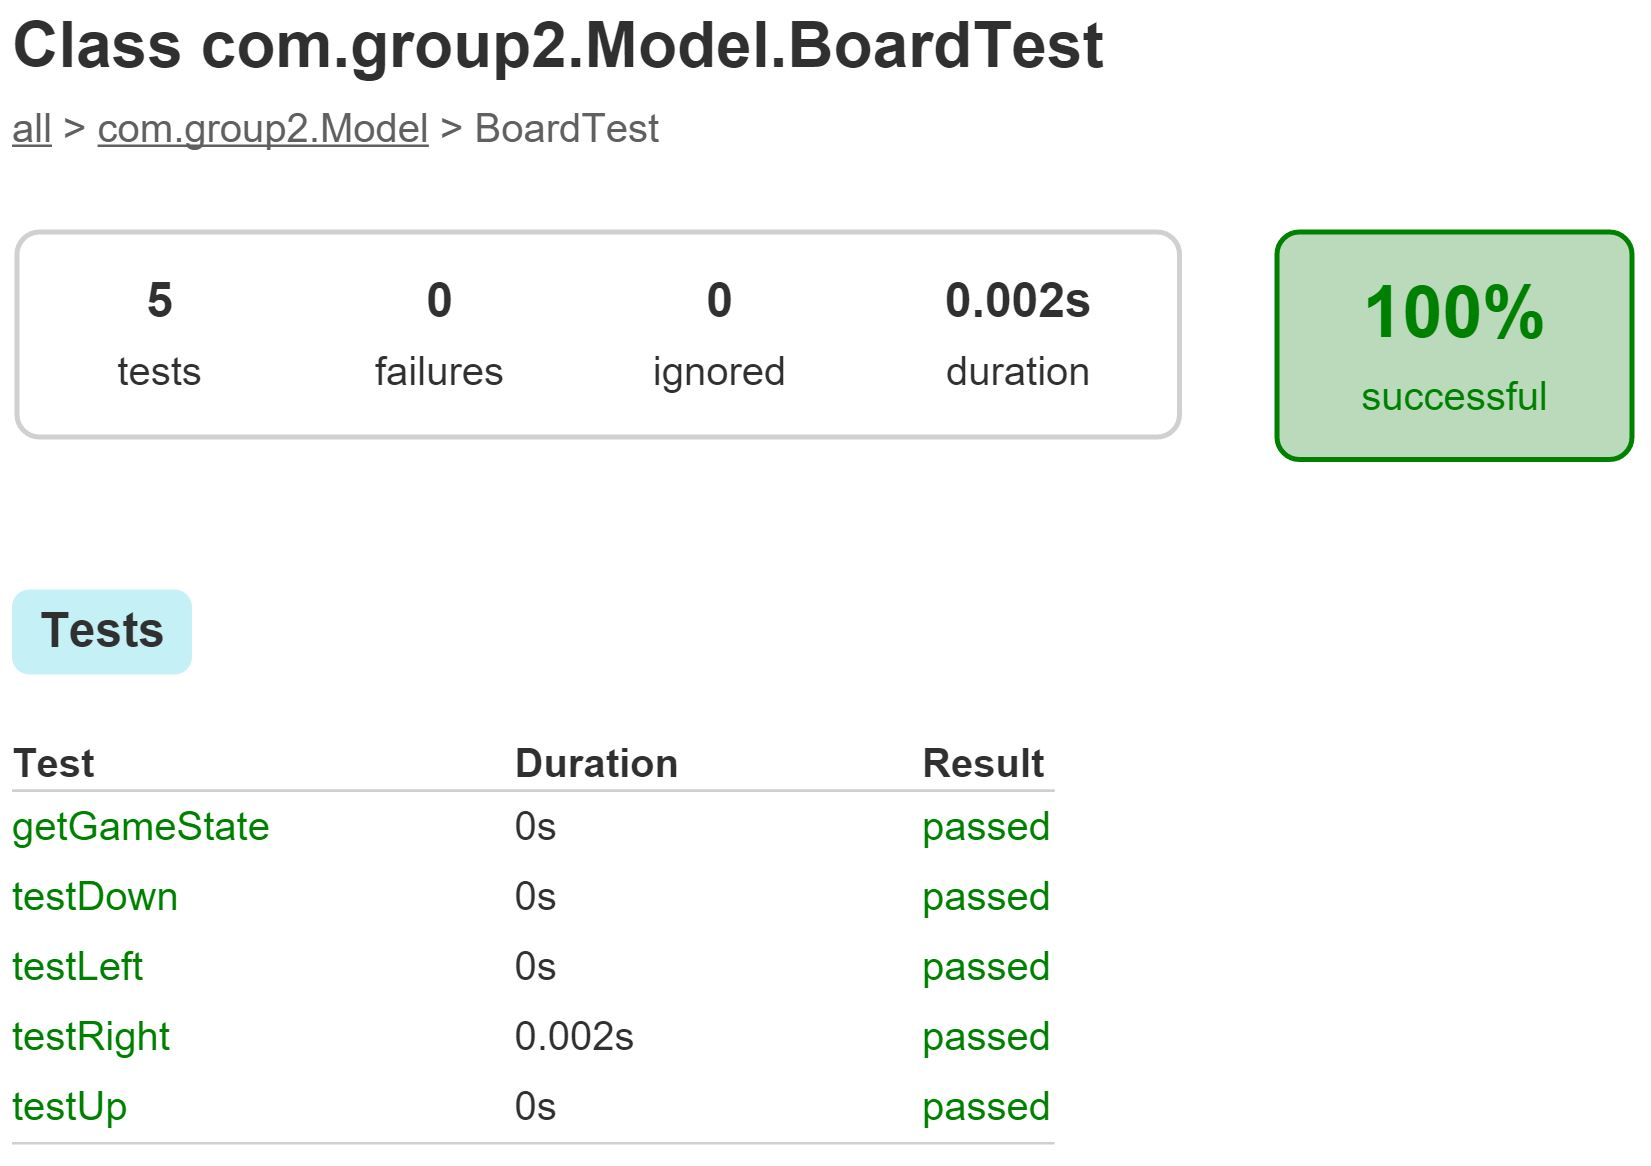
\includegraphics[width = 14cm]{JUnit_Test_Results}
	\caption{JUnit Test Results}
	\label{JUnit Test Results}
\end{figure}

\end{document}
